\TODO
Hoped for a chip with Spartan-6 LX150T (Støvneng planned for it).
Could not be delivered.
Got SP605 with LX45T instead.
Same architecture, 70\% less logic.
Scalable: Can simply reduce size of sblock matrix.

\section{Spartan-6 SP605 Evaluation Platform}

The Spartan-6 SP605 Evaluation Platform is essentially a board with the Spartan-6 LX45T FPGA wired to every useful peripheral imaginable.
It has connections for PCI Express\footnotemark, Ethernet, DVI, USB, flash card, JTAG, LEDs, switches, and more.
However, the only peripherals utilized in this paper are PCI Express and JTAG.
An overview of the system is shown in \figurename~\ref{fig:sp605}.

\footnotetext {
    Even though the PCI Express finger has lines for power, they are not connected on the SP605.
    This means an external power source has to be connected.
}

\begin{figure}[!ht]
    \centering
    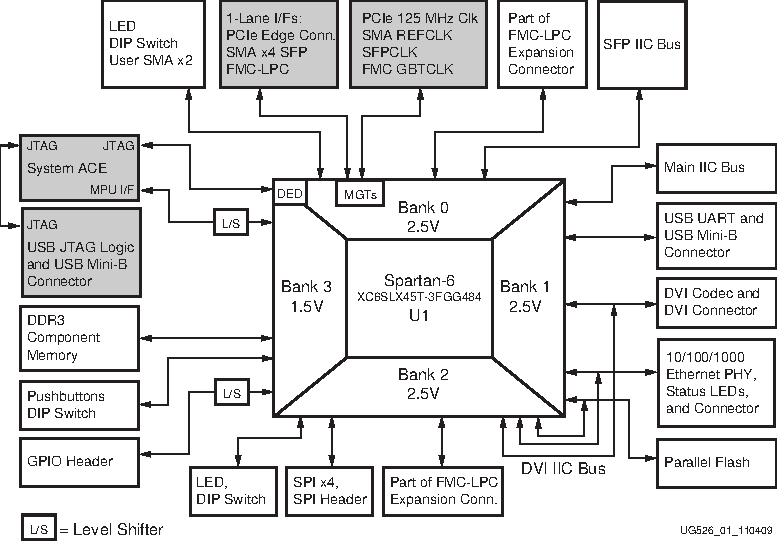
\includegraphics[width=\textwidth]{figures/sp605-modified}
    \caption[SP605]{
        High-level block diagram of the SP605 and its peripherals.
        Peripherals utilized in this paper are highlighted in gray.
        (Modified reprint from \cite{ug526})
    }
    \label{fig:sp605}
\end{figure}

The Spartan-6 is Xilinx' most cost-effective FPGA series.
Its CLBs are divided into two independent slices, one of which is connected to a carry-chain.
In addition to the standard slices which contain mainly LUTs and FFs, the Spartan-6 also contains a handful of specialized Digital Signal Processing (DSP) slices.
These are optimized for pipelined wide multiplication and addition, which is required by many signal processing methods.

\section{Hardware Setup}

Due to the experimental nature of testing a new hardware platform, two computers were used in this project, as shown in \figurename~\ref{fig:hardware-setup}.
One is the main development workstation, used for coding and synthesis; it has a JTAG connection to the SP605 over USB, which allows it to upload new designs.
The other is the host for the SP605, which is mounted in a PCI Express expansion slot.

\begin{figure}[!ht]
    \centering
    
\includegraphics[width=32\block]{figures/hardware-setup}
    \caption[Hardware setup]{
        High-level block diagram of the hardware setup.
    }
    \label{fig:hardware-setup}
\end{figure}

The setup allows a new design to be uploaded and tested on the SP605 without disrupting the workflow of the main workstation due to the power-cycle required to reset the PCI Express connection after a new design has been uploaded.

The switch and jumper configurations of the SP605 are set to factory defaults per \cite{ug526}, with the exception of SW1 which is set to 10 (M0=1 and M1=0).

\section{Software Setup}

The operating systems used on the computers have varied, without complications, between Linux Mint 16, Linux Mint 17 and Manjaro during the lifespan of the project.
Linux Mint and Ubuntu, which it is based upon, are currently the two most popular Linux distributions \cite{distrowatch}.
Manjaro and its base Arch has a lot smaller user base, but is popular with enthusiasts.
The procedures and software used in this paper should therefore work without trouble on most Linux systems.

Xilinx ISE version 13.3 was used for hardware design and synthesis, while ISim was used for simulations.
The third-party USB cable driver from \cite{usbdriver} was used for JTAG, as explained in Section~\ref{sec:challenges}.
The software API was compiled with both GCC version 4.8.2 and 4.9.2.

